\documentclass[11pt]{article}
\usepackage[T1]{fontenc}
\usepackage[utf8]{inputenc}
\usepackage[a4paper,margin=0.9in]{geometry}
\usepackage{textcomp}
\usepackage{booktabs}
\usepackage{multirow}
\usepackage{array}
\usepackage{amsmath,amssymb}
\usepackage{float}
\usepackage{graphicx}
\usepackage{caption}
\usepackage{subcaption}
\usepackage{xcolor}
\usepackage{hyperref}
\hypersetup{colorlinks=true,linkcolor=blue!50!black,urlcolor=blue!50!black,
            linktoc=all,bookmarksopen=true,bookmarksopenlevel=1}
\setlength{\parindent}{0pt}
\setlength{\parskip}{6pt}

\title{Electoral Turnover and Forest Cover in Brazil:\\
       Close-Elections RD Estimates for Three Forest Outcomes}
\author{Generated by \texttt{run\_rd\_brasil.py}}
\date{\today}
\begin{document}\maketitle
\tableofcontents
\clearpage


\section{Data and outcome construction}

\subsection{Pipeline}

Three production stages: (i)~a Python data builder
(\texttt{B\_codes/build\_rd\_panel\_brasil.py}) that consumes TSE election
data (via BigQuery / Base dos Dados), MapBiomas Collection~10 forest layers,
and MODIS VCF tree cover, and writes
\texttt{rd\_panel\_turnover\_bosque.csv} (one row per municipality-election);
(ii)~this analysis script (\texttt{run\_rd\_brasil.py}) that constructs the
five MPR horizons, estimates the RD via \texttt{rdrobust}, runs the McCrary
density test via \texttt{rddensity}, and generates rdplots;
(iii)~this report, assembled automatically by the same script.

\subsection{Outcomes ($K=3$)}

Three forest-cover measures, each averaged at the municipality level:

\begin{itemize}
  \item \texttt{native\_mb} --- MapBiomas Collection~10 native forest
        (\texttt{forest\_native\_ha}), annual area in hectares, 2000--2024.
  \item \texttt{formation\_mb} --- MapBiomas Collection~10 forest formation
        (\texttt{forest\_formation\_ha}), annual area in hectares, 2000--2024.
  \item \texttt{treecover\_modis} --- MODIS VCF (MOD44B v061)
        \texttt{Percent\_Tree\_Cover}, municipality-level mean, 2000--2024.
\end{itemize}

\subsection{Marx--Pons--Rollet $\Delta Y$ construction}

For each (municipality $m$, election year $t$),
\[
\Delta Y^{\text{main}}_{m,t}
  \;=\; \tfrac{1}{4}\sum_{\tau=1}^{4} Y_{m,t+\tau}
  \;-\; Y_{m,t-1},
\]
the post-election four-year mean minus the pre-election value. Shorter
horizons replace the $1/4$ post-mean by $1/k$ for $k\in\{1,2,3\}$; the
\texttt{pre3} robustness spec replaces $Y_{m,t-1}$ with the mean of
$Y_{m,t-3..t-1}$. All $\Delta Y$ are $z$-standardised using the
$(\mu,\sigma)$ from the full main-horizon sample.


\subsection{The RD design}

\begin{itemize}
\item \textbf{Running variable.} $\text{score} = \text{margin} \times
  \widetilde{\text{turnover}}$, where margin $=$ vote share of the winner
  $-$ vote share of the runner-up, and
  $\widetilde{\text{turnover}} = +1$ if the winning party changed
  (turnover) and $-1$ if the same party re-won (continuity).
\item \textbf{Treatment at the cutoff.} Party-level mayoral turnover in a
  close election. Positive score $\to$ turnover; negative $\to$ continuity.
\item \textbf{Sample.} Brazilian municipal elections 2000, 2004, 2008, 2012, 2016, 2020, 2024
  (5,568 municipalities, 32,453 muni-election cells with valid
  running variable). Average turnover rate: $\bar T = 0.725$.
\item \textbf{Estimator.} \texttt{rdrobust} with $p=1$, triangular kernel,
  MSE-optimal bandwidth (\texttt{bwselect("mserd")}). Reported: bias-corrected
  point estimate with robust SE and $p$-value (``Robust'' line).
\end{itemize}

\clearpage


\section{RD results}

\subsection{Main results table}

\begin{table}[H]
\centering
\scriptsize
\caption{RD estimates: turnover $\to$ forest cover (Brazil). Per-cell:
bias-corrected coefficient (top), robust SE (parentheses), MSE-optimal
bandwidth $h$, and effective number of observations $N_h$. $p=1$,
triangular kernel.}
\label{tab:rd_brasil}
\begin{tabular}{l ccc ccc ccc}
\toprule

 & \multicolumn{3}{c}{\texttt{Native forest (MB)}} & \multicolumn{3}{c}{\texttt{Forest form. (MB)}} & \multicolumn{3}{c}{\texttt{Tree cover (MODIS)}} \\
\cmidrule(lr){2-4} \cmidrule(lr){5-7} \cmidrule(lr){8-10}
Horizon & Coef. & $h$ & $N_h$ & Coef. & $h$ & $N_h$ & Coef. & $h$ & $N_h$ \\
\midrule
$\Delta Y^{\text{main}}$ & -0.061$^{**}$ & 13.99 & 16,047 & -0.036 & 14.34 & 16,333 & -0.070$^{*}$ & 14.45 & 16,413 \\
 & (0.031) &  &  & (0.030) &  &  & (0.042) &  &  \\
\addlinespace[1pt]
$\Delta Y^{k=1}$ & -0.055$^{*}$ & 13.22 & 15,474 & -0.028 & 13.60 & 15,744 & -0.025 & 16.20 & 17,665 \\
 & (0.031) &  &  & (0.030) &  &  & (0.041) &  &  \\
\addlinespace[1pt]
$\Delta Y^{k=2}$ & -0.055$^{*}$ & 13.25 & 15,489 & -0.030 & 13.45 & 15,628 & -0.038 & 15.47 & 17,164 \\
 & (0.031) &  &  & (0.030) &  &  & (0.041) &  &  \\
\addlinespace[1pt]
$\Delta Y^{k=3}$ & -0.058$^{*}$ & 13.75 & 15,865 & -0.033 & 13.84 & 15,941 & -0.063 & 14.49 & 16,444 \\
 & (0.031) &  &  & (0.030) &  &  & (0.043) &  &  \\
\addlinespace[1pt]
$\Delta Y^{\text{pre}_3}$ & -0.061$^{**}$ & 14.83 & 16,715 & -0.036 & 14.93 & 16,784 & -0.043 & 16.18 & 17,657 \\
 & (0.030) &  &  & (0.030) &  &  & (0.041) &  &  \\
\addlinespace[1pt]
\midrule
McCrary $p_q$ & \multicolumn{3}{c}{0.000$\dagger$} & \multicolumn{3}{c}{0.000$\dagger$} & \multicolumn{3}{c}{0.000$\dagger$} \\
\bottomrule
\end{tabular}
\begin{flushleft}\footnotesize
\textit{Notes.} Stars on the RD coefficient: $^{*}p<0.10$,
$^{**}p<0.05$, $^{***}p<0.01$ (robust $p$-value).
$\dagger$ Marker on McCrary $p_q<0.10$: weak evidence of running-variable
manipulation at the cutoff.\\
\end{flushleft}
\end{table}


\clearpage
\subsection{RD plots (main horizon)}

\begin{figure}[H]
\centering
\begin{subfigure}{0.32\linewidth}%
  \centering%
  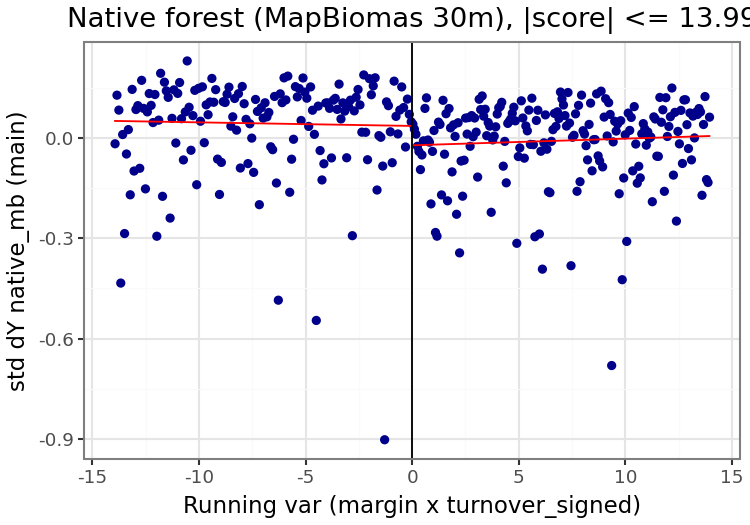
\includegraphics[width=\linewidth]{figs/rdplot_native_mb.png}%
  \caption*{\small Native forest (MapBiomas 30m)}%
\end{subfigure}\hfill%
\begin{subfigure}{0.32\linewidth}%
  \centering%
  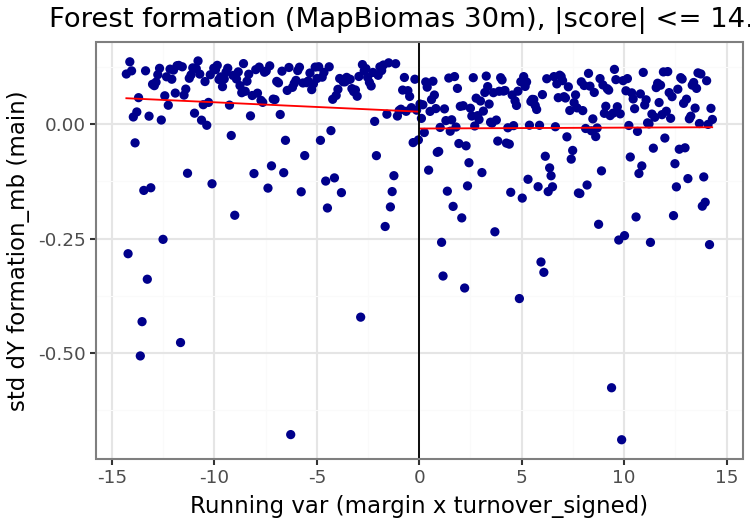
\includegraphics[width=\linewidth]{figs/rdplot_formation_mb.png}%
  \caption*{\small Forest formation (MapBiomas 30m)}%
\end{subfigure}\hfill%
\begin{subfigure}{0.32\linewidth}%
  \centering%
  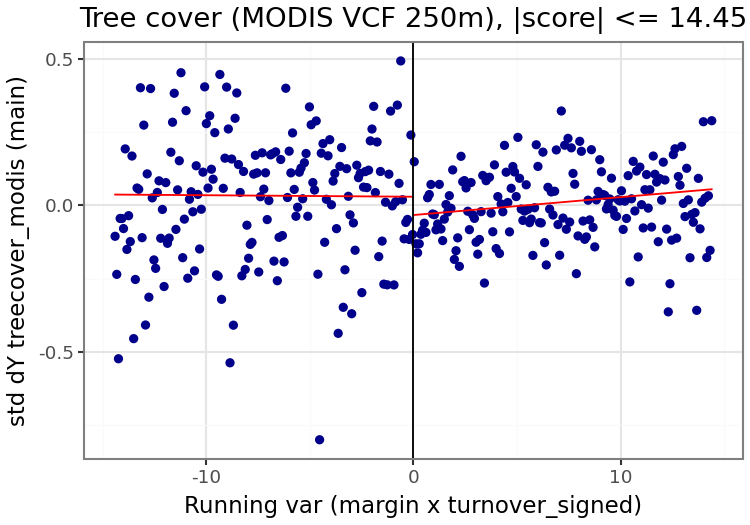
\includegraphics[width=\linewidth]{figs/rdplot_treecover_modis.png}%
  \caption*{\small Tree cover (MODIS VCF 250m)}%
\end{subfigure}%
\caption{RD plots for the three forest outcomes (main horizon),
restricted to the MSE-optimal bandwidth. Score:
$\text{margin}\times\widetilde{\text{turnover}}$, binselect = esmv.}
\label{fig:rdplots_brasil}
\end{figure}


\clearpage
\subsection{McCrary density tests}

\begin{table}[H]
\centering
\small
\caption{McCrary (rddensity) test on the running variable at the cutoff ($c=0$).
$H_0$: no manipulation. $\dagger$ flags $p_q<0.10$.}
\label{tab:mccrary_brasil}
\begin{tabular}{l rrrr}
\toprule
Outcome & $T_q$ & $p_q$ & $N_l$ & $N_r$ \\
\midrule

\texttt{native\_mb} & 18.416 & 0.000$\dagger$ & 7,217 & 19,790 \\
\texttt{formation\_mb} & 18.416 & 0.000$\dagger$ & 7,217 & 19,790 \\
\texttt{treecover\_modis} & 18.416 & 0.000$\dagger$ & 7,217 & 19,790 \\
\bottomrule
\end{tabular}
\end{table}


\end{document}
